
\section{Results and Discussion}

\begin{raggedright}
\subsection{Tag-based regulation improves problem-solving performance on context-dependent tasks}
\end{raggedright}

% Overview paragraph (outline results across all three context-dependent problems)
We found that tag-based regulation improves performance on each of the three problems that require context-dependent behavior: the signal-counting problem (Section \ref{chapter:tag-based-regulation:sec:results:signal-counting-problem}), contextual-signal problem (Section \ref{chapter:tag-based-regulation:sec:results:context-signal-problem}), and Boolean-logic calculator problem (Section \ref{chapter:tag-based-regulation:sec:results:boolean-calc-problem}). 
Additionally, we conducted knockout experiments that confirmed that evolved tag-based regulation allows solutions to dynamically adjust module execution over time. 
We also found that, across all three context-dependent problems, regulation-off solutions (\textit{i.e.}, solutions evolved using regulation-disabled SignalGP) executed a larger proportion of conditional logic instructions than regulation-on solutions (\textit{i.e.}, solutions evolved using regulation-enabled SignalGP). 
This result suggests that without regulation, programs must evolve larger, more complex conditional logic structures. 

\subsubsection{Signal-counting Problem}
\label{chapter:tag-based-regulation:sec:results:signal-counting-problem}


\begin{table}[ht!]
    \small
    \centering
    \begin{tabularx}{\columnwidth}{cYY}
        \toprule
          & Regulation-off condition 
          & Regulation-on condition \\
        %  \hline
        \cmidrule(lr){1-3}
         Two-signal   
            & \RSPTwoSigMemOnlySolutionCnt  % Memory-only
            & \RSPTwoSigBothSolutionCnt \\  % Both
        %  \hline
         Four-signal
            & \RSPFourSigMemOnlySolutionCnt  % Memory-only
            & \RSPFourSigBothSolutionCnt \\  % Both
        %  \hline
         Eight-signal 
            & \RSPEightSigMemOnlySolutionCnt  % Memory-only
            & \RSPEightSigBothSolutionCnt \\  % Both
        %  \hline
         Sixteen-signal
            & \RSPSixteenSigMemOnlySolutionCnt  % Memory-only
            & \RSPSixteenSigBothSolutionCnt \\  % Both
         \bottomrule
    \end{tabularx}
    \caption{\small
    \textbf{Signal-counting problem-solving success.}
    This table gives the number of successful replicates (\textit{i.e.}, in which a perfect solution evolved) out of 200 on the signal-counting problem across four problem difficulties and two experimental conditions. 
    For each problem difficulty, the regulation-off condition was less successful than the regulation-on condition (Fisher's exact test; all difficulties: $p < 10^{-15}$).
    }
    \label{chapter:tag-based-regulation:tab:signal-counting-solutions}
\end{table}


% two-signal: p-value < 2.2e-16, 
% four-signal: p-value < 2.2e-16
% eight-signal: p-value < 2.2e-16
% sixteen-signal: p-value < 2.2e-16

% (1) # Solution & solution timing
Table \ref{chapter:tag-based-regulation:tab:signal-counting-solutions} shows the results from the signal-counting problem for each experimental condition across all four levels of problem difficulty. 
Regulation-on conditions consistently yielded a larger number of successful replicates than regulation-off conditions where programs relied on their global memory buffer in combination with procedural flow control for success.
Although global memory is technically sufficient to solve each version of the signal-counting problem\footnote{
We verified this claim by hand-coding solutions that rely on global memory and flow-control instructions (supplemental \supSecHandcodedPrograms\ \citep{tag_regulation_supplement_2021}).
}, 
in practice such solutions evolved in only the two- and four-signal variants.
Tag-based regulation, in contrast, appears more readily adaptive, as regulation-based solutions arose across all problem difficulties, implying that access to tag-based regulation can drive increased problem-solving success.
Further, we found that, in the two- and four-signal tasks, solutions arose after significantly fewer generations in the regulation-on conditions than in the regulation-off controls (Figure \ref{chapter:tag-based-regulation:fig:signal-counting-solve-time}).


\begin{figure}[htbp]
    \centering
    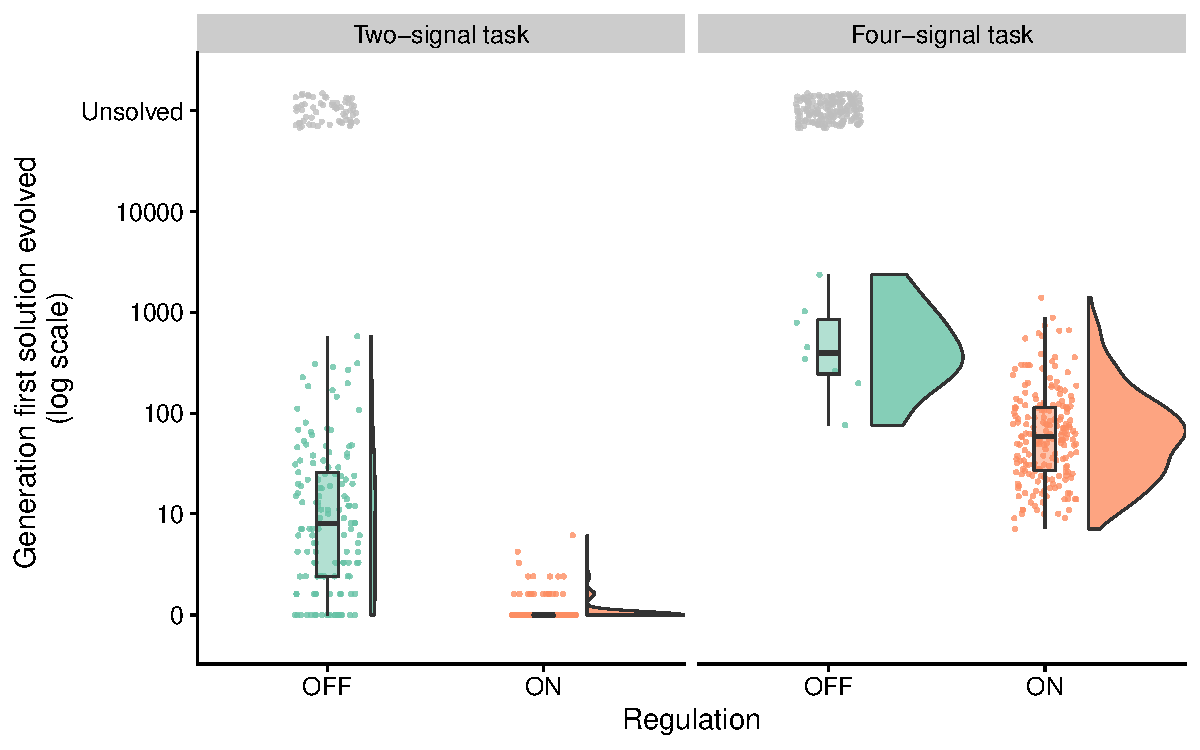
\includegraphics[width=0.7\textwidth]{chapters/05-tag-based-genetic-regulation/media/signal-counting-solve-time-cloud.pdf}
    \caption{\small
    \textbf{Generation at which first solution evolved (log scale) in each successful replicate for the signal-counting problem (raincloud plot \citep{allen_raincloud_2019}).}
    We show data from only those problem difficulties in which solutions evolved (two- and four-signal problems).
    Gray points indicate the number of unsuccessful replicates for each condition.
    For both problem difficulties, regulation-on solutions typically required fewer generations than regulation-off solutions to arise (Wilcoxon rank sum test; two-signal: $p < 10^{-15}$, four-signal: $p < 9\times10^{-05}$). 
    }
    \label{chapter:tag-based-regulation:fig:signal-counting-solve-time}
\end{figure}

% two-signal - p-value < 2.2e-16
% four-signal 8.603e-05

Tag-based regulation renders the two-signal task trivial: all solutions evolved in under 10 generations. 
In fact, the majority of regulation-on solutions (178 out of 200) were found in the initial randomly generated population. 
However, not all replicates without access to tag-based regulation even found a solution to the two-signal task.

\begin{table}[htbp]
    \small
    \centering
    \begin{tabularx}{\columnwidth}{cYYY}
        \toprule
          & No regulation required
          & Regulation required 
          & Unsolved \\
        %  \hline
        \cmidrule(lr){1-4}
         Two-signal     
            & \RSPTwoSigMemOnlyStrategyCnt  % Memory-only
            & \RSPTwoSigRegRequiredStrategyCnt  
            & \RSPTwoSigUnsolvedCnt \\
        %  \hline
         Four-signal    
            & \RSPFourSigMemOnlyStrategyCnt  % Memory-only
            & \RSPFourSigRegRequiredStrategyCnt   % 
            & \RSPFourSigUnsolvedCnt \ \\
        %  \hline
         Eight-signal   
            & \RSPEightSigMemOnlyStrategyCnt  % Memory-only
            & \RSPEightSigRegRequiredStrategyCnt  % 
            & \RSPEightSigUnsolvedCnt \\
        %  \hline
         Sixteen-signal 
            & \RSPSixteenSigMemOnlyStrategyCnt  % Memory-only
            & \RSPSixteenSigRegRequiredStrategyCnt  % 
            & \RSPSixteenSigUnsolvedCnt \\
         \bottomrule
    \end{tabularx}
    \caption{\small 
    \textbf{Mechanisms underlying solutions from the regulation-on condition for the signal-counting problem.}
    To determine a successful program's underlying strategy, we re-evaluated the program with global memory access instructions knocked out (\textit{i.e.}, replaced with no-operation instructions) and with regulation instructions knocked out.
    This table shows the number of regulation-on solutions that actually rely on regulation to solve the signal-counting problem. 
    }
    \label{chapter:tag-based-regulation:tab:signal-counting-ko-strategies}
\end{table} 

We conducted knockout experiments to investigate the mechanisms underlying successful programs. 
Indeed, all solutions evolved without access to tag-based regulation relied exclusively on their global memory buffer to differentiate their behavior (see supplemental \supSecRepeatedSigAnalysis\ \citep{tag_regulation_supplement_2021}). 
Table \ref{chapter:tag-based-regulation:tab:signal-counting-ko-strategies} shows the strategies used by programs evolved with regulation-enabled SignalGP.
Our knockout experiments confirm that the majority of solutions evolved with access to tag-based regulation do indeed rely on regulation to dynamically adjust their responses to signals over time. 


\begin{figure}[ht]
\centering

\begin{subfigure}[b]{0.55\textwidth}
    \centering
    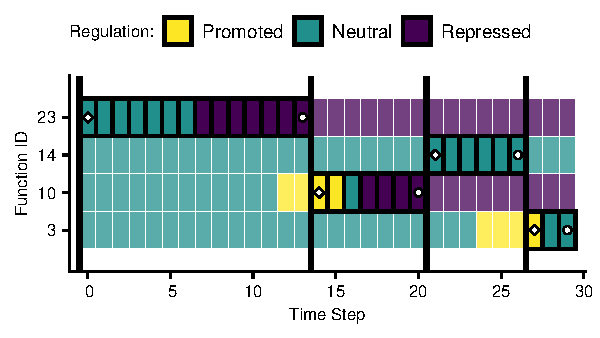
\includegraphics[width=\linewidth]{chapters/05-tag-based-genetic-regulation/media/signal-counting-networks/case-study-trace-id-20203-regulator-state-horizontal.pdf}
    \caption{\small Module regulation over time.}
    \label{chapter:tag-based-regulation:subfig:rst-exec-trace}
\end{subfigure}%
\hfill
\begin{subfigure}[b]{0.3\textwidth}
    \centering
    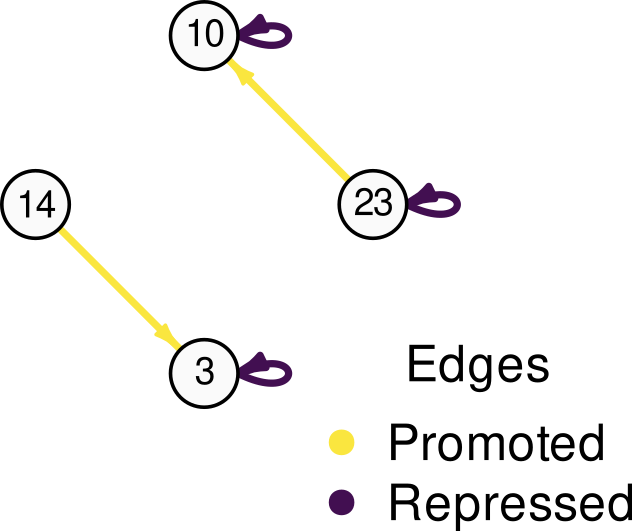
\includegraphics[width=\linewidth]{chapters/05-tag-based-genetic-regulation/media/signal-counting-networks/case-study-id-20203-network.png}
    \caption{\small Regulatory network.}
    \label{chapter:tag-based-regulation:subfig:rst-reg-network}
\end{subfigure}%


\caption{\small 
   \textbf{Execution trace of a SignalGP program solving the four-signal version of the signal-counting task.}
    Color denotes each function's regulatory state (yellow: promoted, purple: repressed) during evaluation; functions not regulated or executed are omitted.
    Functions that are actively executing are annotated with a black outline.
    Black vertical lines denote input signals, and a diamond (white with black outline) indicates which function was triggered by the input signal.
    A circle (white with black outline) indicates which function executed a response.
    (b) shows the directed graph representing the regulatory network associated with trace (a).
    Vertices depict functions that either ran during evaluation or were regulated. 
    Each directed edge shows a regulatory relationship between two functions where the edge's source acted on (promoted in yellow or repressed in purple) the edge's destination.
    Note that in the case presented here all repressing relationships are self-referential.
    }
    
\label{chapter:tag-based-regulation:fig:signal-counting-example-networks}
\end{figure}


% (3) Evolved networks
We further assessed the functionality of tag-based regulation by analyzing the execution traces of evolved solutions.
We visualized the gene regulatory networks that manifest as a result of programs executing promoter and repressor instructions. 
Figure \ref{chapter:tag-based-regulation:fig:signal-counting-example-networks} overviews the execution of a representative evolved program on the four-signal instance of the signal-counting problem.
We found that successful programs tend to operate via a succession of self-repressing events where modules express the appropriate response then disable themselves so that the next best-matching function---expressing the appropriate next response---will activate instead.
This behavioral pattern continues for each subsequent environmental signal.
Indeed, across all problem difficulties, we observed that successful regulatory networks generally contained more repression relationships than promotion relationships between functions (supplemental \supSecRepeatedSigAnalysis\  \citep{tag_regulation_supplement_2021}).
Independent knockouts of up-regulation and down-regulation confirm that the majority of successful regulatory networks rely on down-regulation: 
of the 661 successful regulatory networks evolved across all problem difficulties, 392 rely exclusively on down-regulation, 7 rely exclusively on up-regulation, 259 rely on both up- and down-regulation, and 3 rely on \textit{either} up- or down-regulation (\textit{i.e.}, they required regulation but were robust to independent knockouts of up- and down-regulation). 

Our experimental data highlights the benefit of tag-based genetic regulation in addition to traditional, register-based means of dynamically adjusting responses to a repeated input signal over time. 
However, our data may also indicate a deficiency in the design of SignalGP's current global memory model.
An improved memory model may also enhance the capacity for programs to dynamically adjust their responses to inputs over time; however, any memory-based solution will still suffer from the need to incorporate flow-control structures to implement this functionality, inherently creating a larger evolutionary hurdle to overcome.
Indeed, we found that the memory-based solutions that evolved in our experiments executed a larger proportion of flow-control instructions than regulation-based solutions
(Wilcoxon rank sum test; two-signal: $p < 10^{-10}$, four-signal: $p = 0.004$; supplemental \supSecRepeatedSigAnalysis\ \citep{tag_regulation_supplement_2021}).
% two-signal: p-value = 2.118e-11; 95% ci 2% to 3.7% difference in proportion
% four-signal: p-value = 0.003185; 95% ci 1.56% to 6.4% difference in proportion

\subsubsection{Contextual-signal Problem}
\label{chapter:tag-based-regulation:sec:results:context-signal-problem}

% (1) Solutions + solution timings

\begin{figure}[ht]
\centering

\begin{subfigure}[b]{0.45\textwidth}
    \centering
    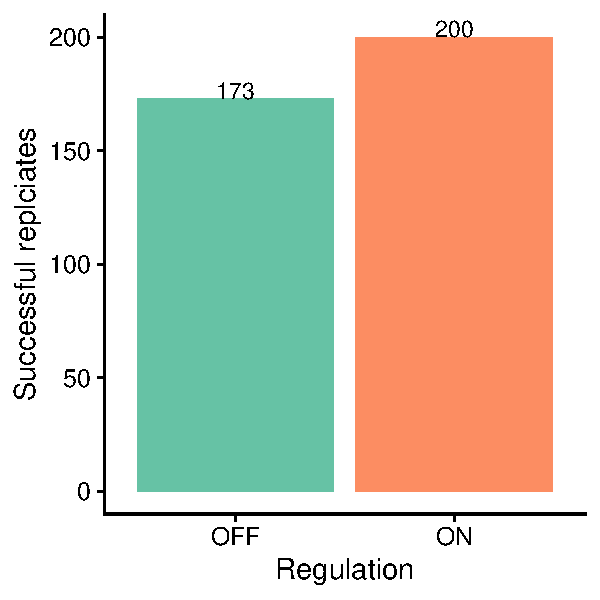
\includegraphics[width=\linewidth]{chapters/05-tag-based-genetic-regulation/media/context-signal-solution-counts.pdf}
    \caption{\small Successful replicates.}
    \label{chapter:tag-based-regulation:subfig:context-signal-solution-counts}
\end{subfigure}
\hfill
\begin{subfigure}[b]{0.45\textwidth}
    \centering
    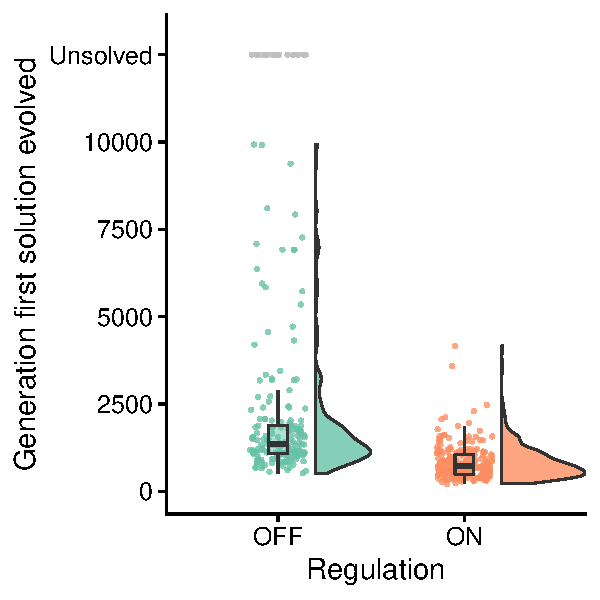
\includegraphics[width=\textwidth]{chapters/05-tag-based-genetic-regulation/media/context-signal-solve-time-cloud.pdf}
    \caption{\small Generations elapsed before solution.}
    \label{chapter:tag-based-regulation:subfig:context-signal-solve-time}
\end{subfigure}

\caption{\small 
\textbf{Contextual-signal problem-solving performance.}
(a) shows the number of successful replicates for the regulation-off and regulation-on conditions on the contextual-signal problem. 
The regulation-off condition was less successful than the regulation-on condition (Fisher's exact test: $p < 6\times10^{-9}$).
(b) is a raincloud plot showing the generation at which the first solution evolved in each successful replicate.
Gray points indicate the number of unsuccessful replicates for each condition.
Regulation-on solutions typically required fewer generations than regulation-off solutions to arise  (Wilcoxon rank sum test: $p < 10^{-15}$).
}

% problem-solving success - p-value = 5.818e-09; fisher's
% solve time: p-value < 2.2e-16; wilcoxon
    
\label{chapter:tag-based-regulation:fig:context-signal-performance}
\end{figure}


Figure \ref{chapter:tag-based-regulation:subfig:context-signal-solution-counts} shows the number of successful replicates on the contextual-signal problem for both the regulation-on and regulation-off conditions.
While both conditions were often successful, we found that access to tag-based regulation significantly improved problem-solving success.
Further, regulation-on solutions typically required fewer generations to evolve than regulation-off solutions (Figure \ref{chapter:tag-based-regulation:subfig:context-signal-solve-time}).

% (2) Solution strategies (knockouts)
We used knockout experiments to identify the mechanisms underlying each solution's strategy.
As expected, all 173 solutions evolved without access to tag-based regulation relied on their global memory buffer to track contextual information and used control flow mechanisms to differentiate their responses based on stored context.
Indeed, we found that regulation-off solutions executed a larger proportion of flow-control instructions than regulation-on solutions (Wilcoxon rank sum test: $p < 10^{-15}$; supplement \supSecContextSigAnalysis\ \citep{tag_regulation_supplement_2021}).
We also found that all 200 regulation-on solutions relied on tag-based regulation for response differentiation: 105 relied only on tag-based regulation and 95 relied on a combination of both tag-based regulation and global memory.
% Control flow proportions:
% p < p-value < 2.2e-16; 95% ci: 4.28% - 5.43%

In contrast to the signal-counting problem, we did not find that successful regulatory networks used primarily self-repressing modules.
Instead, we found that networks were more balanced between repressing and promoting edges; indeed, we found that successful networks generally contained more promoting edges than repressing edges (supplement \supSecContextSigAnalysis\ \citep{tag_regulation_supplement_2021}).
This result suggests that we should expect different problems to select for different forms of gene regulatory networks.

\subsubsection{Boolean-logic Calculator Problem}
\label{chapter:tag-based-regulation:sec:results:boolean-calc-problem}

% (1) solutions + solution timings

\begin{figure}[ht]
\centering

\begin{subfigure}[b]{0.45\textwidth}
    \centering
    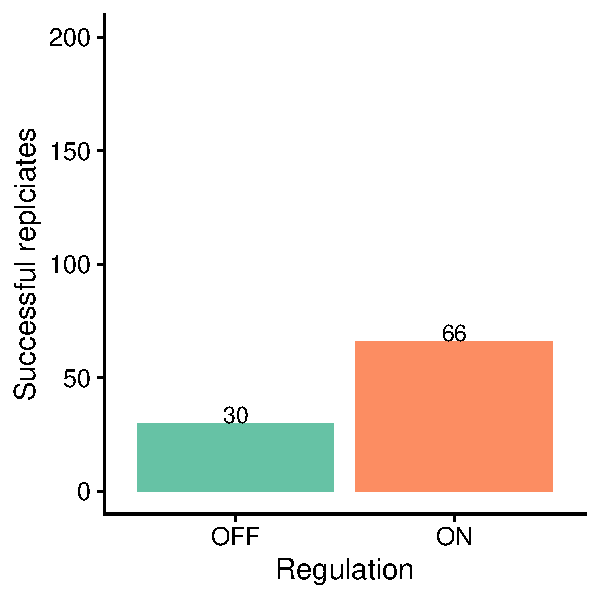
\includegraphics[width=\linewidth]{chapters/05-tag-based-genetic-regulation/media/boolean-calc-prefix-solution-counts.pdf}
    \caption{\small Successful replicates.}
    \label{chapter:tag-based-regulation:subfig:boolean-calc-prefix-solution-count}
\end{subfigure}
\hfill
\begin{subfigure}[b]{0.45\textwidth}
    \centering
    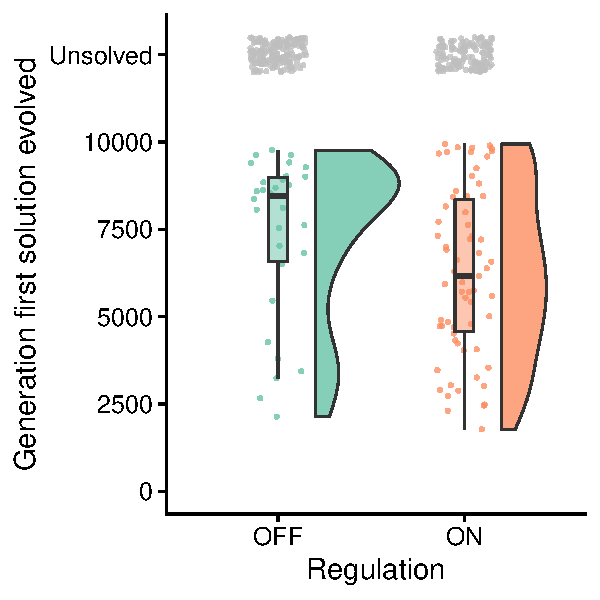
\includegraphics[width=\textwidth]{chapters/05-tag-based-genetic-regulation/media/boolean-calc-prefix-solve-time-cloud.pdf}
    \caption{\small Generations elapsed before solution.}
    \label{chapter:tag-based-regulation:subfig:boolean-calc-prefix-solve-time}
\end{subfigure}

\caption{\small
\textbf{Boolean-logic calculator problem-solving performance.}
(a) shows the number of successful replicates for the regulation-off and regulation-on conditions on the Boolean-logic calculator problem. 
The regulation-off condition was less successful than the regulation-on condition (Fisher's exact test: $p < 4\times10^{-05}$).
(b) is a raincloud plot showing the generation at which the first solution evolved in each successful replicate.
Gray points indicate the number of unsuccessful replicates for each condition.
Regulation-on solutions typically required fewer generations than regulation-off solutions to arise (Wilcoxon rank sum test: $p < 0.042$).
}

% fisher's  p-value = 3.585e-05
% wilcoxon rank sum: p-value = 0.04102
    
\label{chapter:tag-based-regulation:fig:boolean-calc-prefix-performance}
\end{figure}


Figure \ref{chapter:tag-based-regulation:subfig:boolean-calc-prefix-solution-count} shows the number of successful replicates on the Boolean-logic calculator problem for both the regulation-on and regulation-off conditions.
While both regulation-on and regulation-off solutions evolved, we again found that access to genetic regulation significantly improved problem-solving success.
Further, as in the signal-counting and contextual-signal problems, regulation-on solutions typically required fewer generations to evolve than regulation-off solutions (Figure~\ref{chapter:tag-based-regulation:subfig:boolean-calc-prefix-solve-time}).


\begin{figure}
\centering

\begin{subfigure}[b]{0.95\textwidth}
    \centering
    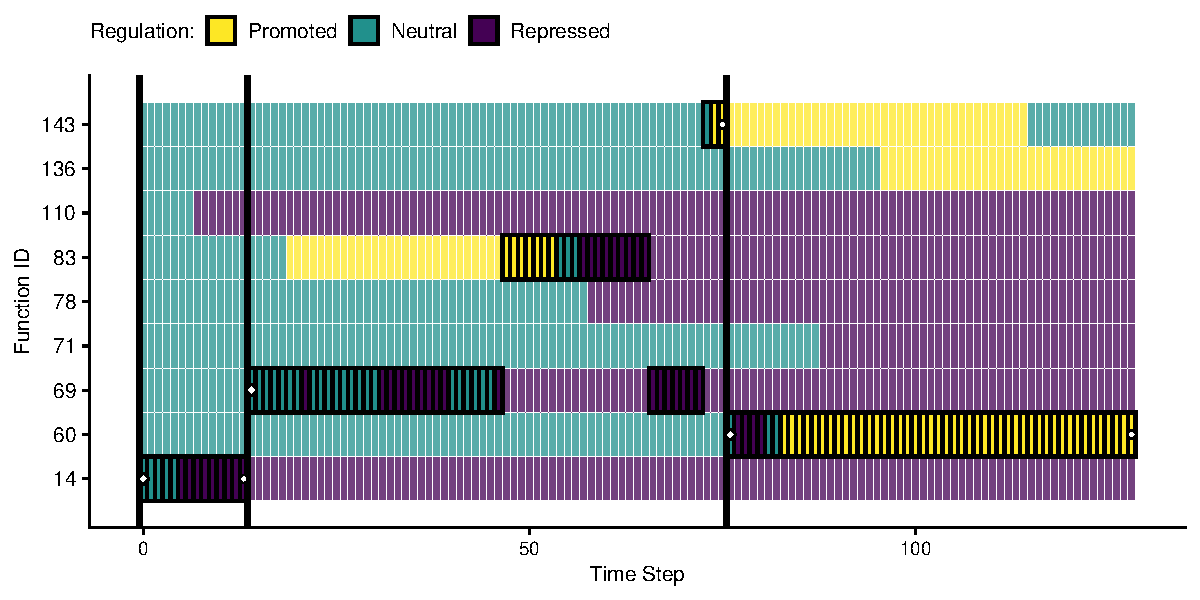
\includegraphics[width=\textwidth]{chapters/05-tag-based-genetic-regulation/media/boolean-calc-prefix-networks/case-study-trace-id-24400-test_id-420-regulator-state-horizontal.pdf}
    \caption{\small  Module regulation over time for a NAND operation.}
    \label{chapter:tag-based-regulation:subfig:bc-nand-exec-trace}
\end{subfigure}%

\begin{subfigure}[b]{0.5\textwidth}
    \centering
    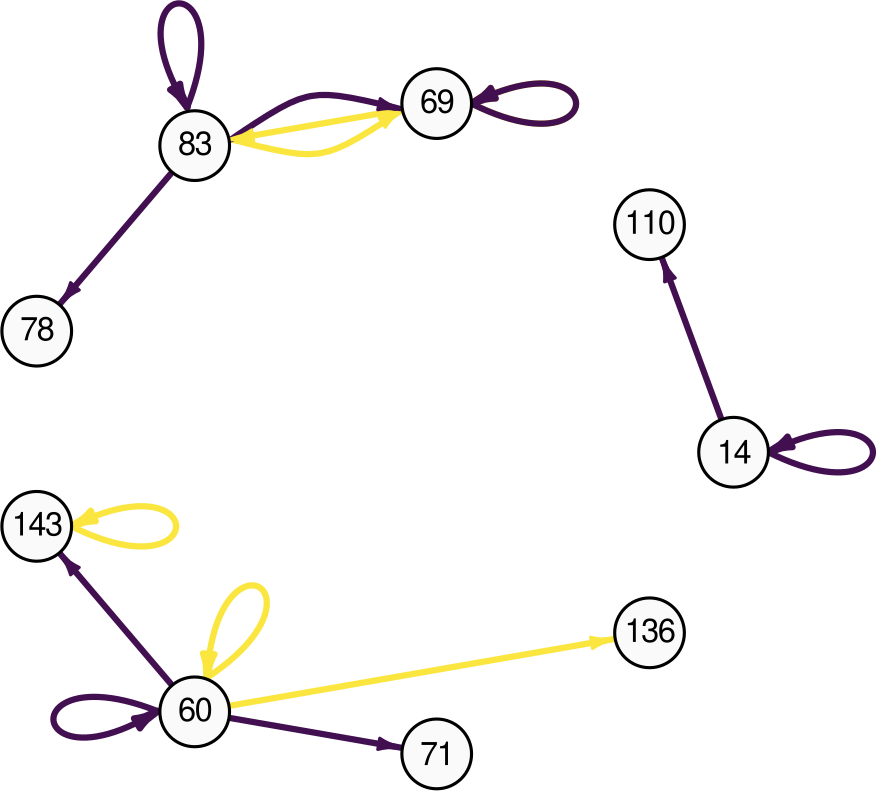
\includegraphics[width=0.6\textwidth]{chapters/05-tag-based-genetic-regulation/media/boolean-calc-prefix-networks/case-study-id-24400-test-420-network-cropped.png}
    \caption{\small NAND regulatory network.}
    \label{chapter:tag-based-regulation:subfig:bc-nand-reg-network}
\end{subfigure}%
\hfill
\begin{subfigure}[b]{0.5\textwidth}
    \centering
    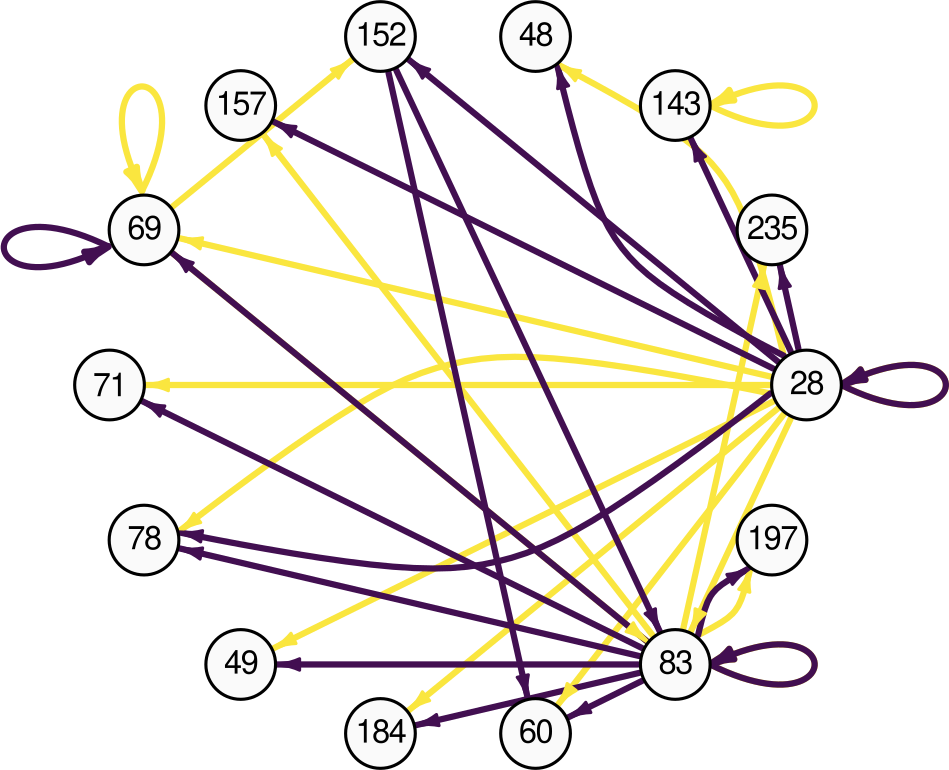
\includegraphics[width=0.6\textwidth]{chapters/05-tag-based-genetic-regulation/media/boolean-calc-prefix-networks/case-study-id-24400-test-134-network-cropped.png}
    \caption{\small NOR regulatory network.}
    \label{chapter:tag-based-regulation:subfig:bc-nor-reg-network}
\end{subfigure}%

\begin{subfigure}[b]{0.95\textwidth}
    \centering
    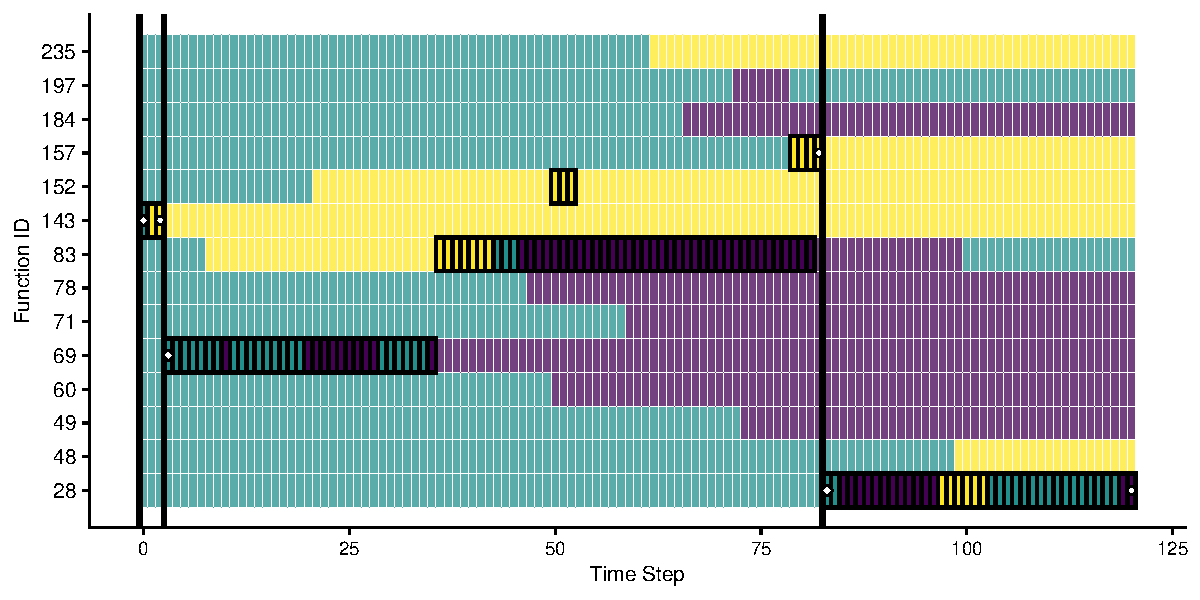
\includegraphics[width=0.95\textwidth]{chapters/05-tag-based-genetic-regulation/media/boolean-calc-prefix-networks/case-study-trace-id-24400-test_id-134-regulator-state-horizontal-nolegend.pdf}
    \caption{\small Module regulation over time for a NOR operation.}
    \label{chapter:tag-based-regulation:subfig:bc-nor-exec-trace}
\end{subfigure}%

\caption{\small 
\textbf{Execution traces of a successful SignalGP program computing a NAND operation (a) and a NOR operation (d).}
(b) and (c) show the directed graphs representing the regulatory networks associated with traces (a) and (d), respectively.
These visualizations are in the same format as those in Figure \ref{chapter:tag-based-regulation:fig:signal-counting-example-networks}.}
\label{chapter:tag-based-regulation:fig:boolean-calc-prefix-example-networks}
\end{figure}


As in previous experiments, we conducted knockout experiments to identify the mechanisms underlying each solution's strategy.
To compute any of the Boolean logic operations, programs \textit{must} make use of the global memory buffer to store numeric inputs (operands) to be used when performing the computation specified by the final operator signal. 
Indeed, all solutions evolved across all conditions relied on their global memory buffer to solve this problem.
All 66 regulation-on solutions, however, also relied on tag-based regulation to perform the appropriate computation for each test case.
Consistent with results from each other context-dependent problem, we found that regulation-off solutions executed a larger proportion of flow-control instructions than regulation-on solutions (Wilcoxon rank sum test: $p < 2\times10^{-05}$; supplement \supSecBooleanCalcPrefixAnalysis\ \citep{tag_regulation_supplement_2021}).
% Wilcoxon rank sum test: p-value = 1.328e-05 CI 1.486% - 3.91%

As in the signal-counting problem, we visualized the gene regulatory networks that manifest as a result of programs executing promoting and repressing instructions. 
Figure \ref{chapter:tag-based-regulation:fig:boolean-calc-prefix-example-networks} overviews the execution of a representative program evolved to solve the Boolean-logic calculator problem.
Specifically, Figure \ref{chapter:tag-based-regulation:fig:boolean-calc-prefix-example-networks} shows a program computing NAND and the same program computing NOR. 
The networks expressed on each of these operations are distinct despite originating from the same code.
These visualizations confirm that tag-based regulation allows programs to dynamically adjust their responses based on context (in this case, an initial operator signal). 

\subsection{Erroneous regulation can hinder task generalization}

In the signal-counting, contextual-signal, and Boolean-logic calculator problems, programs must adjust their behavior depending on the particular sequence of received signals.
The independent-signal problem, however, requires no signal-response plasticity; programs maximize fitness by statically associating $K$ distinct responses each with one of $K$ distinct input signals.
For this task, re-wiring signal-response associations within-lifetime is maladaptive.
As such, does the capacity for regulation impede adaptation to the independent-signal task?

We compared 200 replicate populations evolved with regulation-enabled SignalGP (``regulation-on'') and 200 populations evolved with regulation-disabled SignalGP (``regulation-off'').
All replicates produced a SignalGP program capable of achieving a perfect score during evaluation. 
We found no evidence that the availability of regulation affected the number of generations required to produce these solutions.

Next, we investigated how well evolved solutions \textit{generalized} across random permutations of input sequences.
Selection was deliberately based on a single stochastic ordering of environmental signals, so a ``perfect'' score may not generalize across all signal orderings.
We expect that programs evolved with access to regulation will more often exhibit non-adaptive plasticity that hinders generalization.

Figure \ref{chapter:tag-based-regulation:fig:independent-signal-generalization} shows the number of evolved solutions from each condition that successfully generalized.
All programs that evolved without access to regulation successfully generalized; however, evolved programs from 18 out of 200 successful regulation-on replicates failed to generalize beyond the test cases they experienced during evolution (Fisher's exact test: $p < 6\times10^{-6}$).
Moreover, 5 of 18 non-generalizing programs generalized when we knocked out tag-based regulation.
Upon closer inspection, the other non-general programs relied on tag-based regulation for initial success but failed to generalize to arbitrary environment sequences.
% fisher's p-value = 5.113e-06

\begin{figure}[ht]
    \centering
    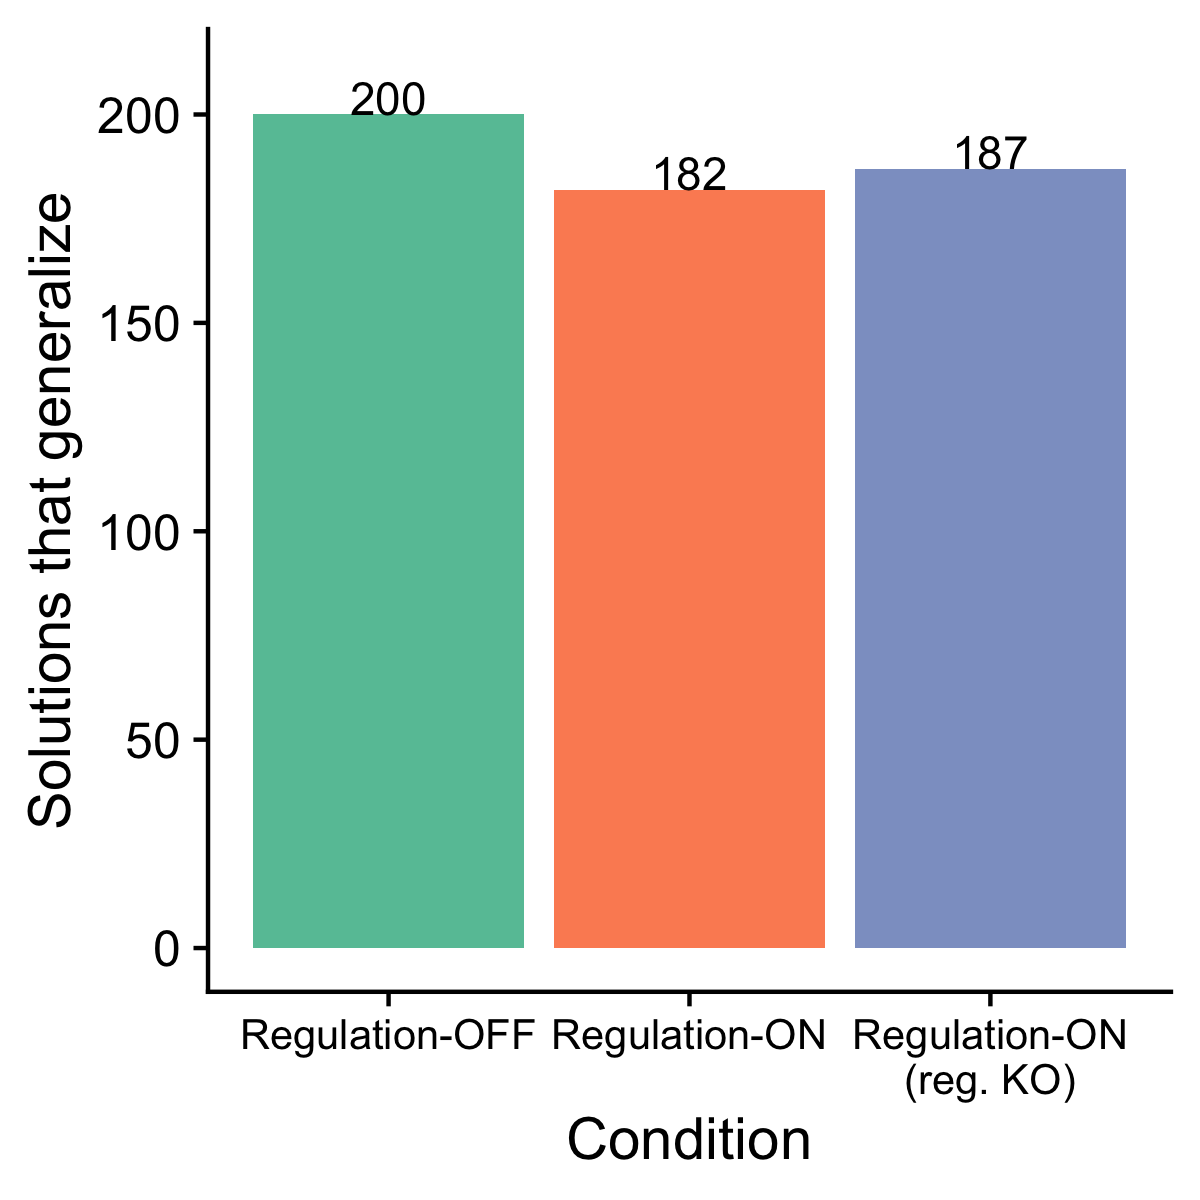
\includegraphics[width=0.5\textwidth]{chapters/05-tag-based-genetic-regulation/media/chg-env-16-generalization.png}
    \caption{\small
    \textbf{The number of evolved solutions that generalize on the independent-signal problem.}
    The difference in number of solutions that generalize between the regulation-on and regulation-off conditions is statistically significant (Fisher's exact test: $p < 6\times10^{-06}$).
    The ``Regulation-ON (reg. KO)'' condition comprises the solutions from the Regulation-on condition, except with regulatory instructions knocked out (\textit{i.e.}, replaced with no-operation instructions).
    }
    \label{chapter:tag-based-regulation:fig:independent-signal-generalization}
\end{figure}




Unexpressed traits that vary in a population (but do not affect fitness) are collectively known as cryptic variation. 
Cryptic variation is pervasive in nature and thought to play an important role in evolution, potentially acting as a cache of diverse phenotypic effects in novel environments \citep{gibson_uncovering_2004,paaby_cryptic_2014}.
Such cryptic variation has been shown to help GP systems escape local optima, improving overall problem-solving performance \citep{turner_neutral_2015}.
Cryptic variation arises when environmental conditions that would reveal the variation are not experienced. 
Access to tag-based regulation appears to make such cryptic variation in evolving programs a stronger possibility than previously.
This dynamic can be valuable for performing more realistic studies of evolutionary dynamics with digital organisms (\textit{i.e.}, self-replicating computer programs \citep{wilke_biology_2002}).
However, when using regulation-enabled SignalGP in problem-solving domains, such as automatic program synthesis, non-adaptive plasticity should be accounted for in fitness objectives.
In the independent-signal problem, for example, we could have performed more thorough evaluations of programs using multiple random permutations of input sequences instead of one.
In more challenging problems, however, more thorough evaluations can come at the cost of substantial computational effort. 

\begin{raggedright}
\subsection{Reducing the context required for the Boolean-logic calculator problem eliminates the benefit of regulation}
\end{raggedright}

Experimental results on the independent-signal problem suggest that enabling tag-based regulation is not necessarily beneficial for solving problems that do not require context-dependent responses to input. 
We use a modified version of the Boolean-logic calculator problem to further investigate the potential for tag-based regulation to impede adaptive evolution. 
The Boolean-logic calculator problem as described in Section \ref{chapter:tag-based-regulation:sec:methods:boolean-calc-problem} provides inputs in prefix notation: the operator (\textit{e.g.}, AND, OR, XOR, \textit{etc.}) is specified first, followed by the requisite number of numeric operands. 
As such, the final input signal does not differentiate which type of computation a program is expected to perform.
Programs must adjust their response based on the context provided by previous signals, thereby increasing the utility of regulation. 

Here, we explore whether the calculator problem's context-dependence is driving the benefit of tag-based regulation that we identified in Section \ref{chapter:tag-based-regulation:sec:results:boolean-calc-problem}.
We can reduce context-dependence of the calculator problem by presenting input sequences in \textit{postfix} notation. 
In postfix notation, programs receive the requisite numeric operand inputs first and the operator input last. 
As such, the final signal in an input sequence will always differentiate which bitwise operation should be performed.
Successful programs must store the numeric inputs embedded in operand signals, and then, as in the independent-signal problem, a distinct signal will differentiate which of the response types a program should execute. 

\begin{figure}[ht]
\centering

\begin{subfigure}[b]{0.45\textwidth}
    \centering
    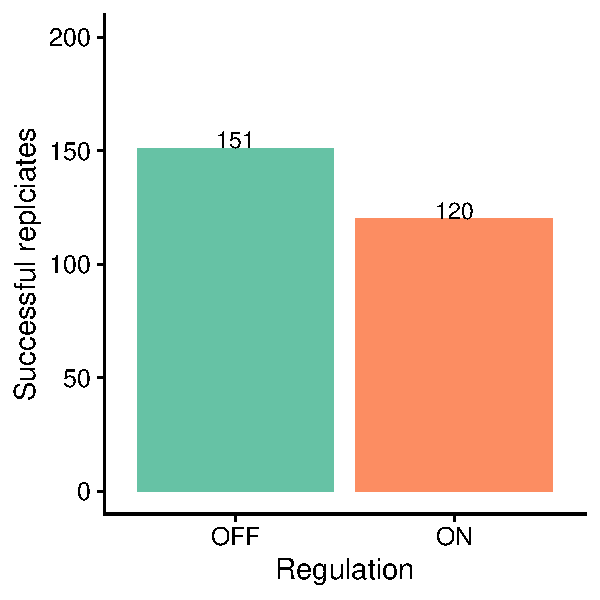
\includegraphics[width=\linewidth]{chapters/05-tag-based-genetic-regulation/media/boolean-calc-postfix-solution-counts.pdf}
    \caption{\small Successful replicates.}
    \label{chapter:tag-based-regulation:subfig:boolean-calc-postfix-solution-count}
\end{subfigure}
\hfill
\begin{subfigure}[b]{0.45\textwidth}
    \centering
    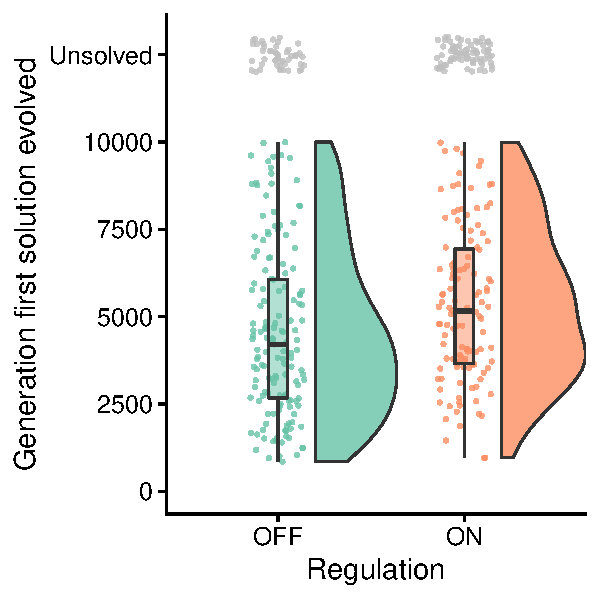
\includegraphics[width=\textwidth]{chapters/05-tag-based-genetic-regulation/media/boolean-calc-postfix-solve-time-cloud.pdf}
    \caption{\small Generations elapsed before solution.}
    \label{chapter:tag-based-regulation:subfig:boolean-calc-postfix-solve-time}
\end{subfigure}

\caption{\small 
\textbf{Boolean-logic calculator (postfix notation)  problem-solving performance.}
(a) shows the number of successful replicates for the regulation-off and regulation-on conditions on the postfix Boolean-logic calculator problem. 
The regulation-on condition was less successful than the regulation-off condition (Fisher's exact test: $p<0.002$).
(b) is a Raincloud plot showing the generation at which the first solution evolved in each successful replicate.
Gray points indicate the unsuccessful replicates for each condition.
Regulation-off solutions typically required fewer generations than regulation-on solutions to arise (Wilcoxon rank sum test: $p<0.004$).
}
% fisher's exact: p-value = 0.001286
% wilcoxon:  p-value = 0.003285
\label{chapter:tag-based-regulation:fig:boolean-calc-postfix-performance}
\end{figure}


We repeated the Boolean-logic calculator experiment (as described in Section \ref{chapter:tag-based-regulation:sec:methods:boolean-calc-problem}), except we presented inputs in postfix notation instead of prefix notation. 
Figure \ref{chapter:tag-based-regulation:subfig:boolean-calc-postfix-solution-count} shows the number of successful replicates evolved in regulation-on and regulation-off conditions.
Postfix notation decreases the overall difficulty of the Boolean-logic calculator problem; more solutions evolved in each condition than evolved with prefix notation (Section \ref{chapter:tag-based-regulation:sec:results:boolean-calc-problem}).
We found that the regulation-on condition resulted in lower problem-solving success than the regulation-off condition. 
We also found that regulation-off solutions typically required fewer generations than regulation-on solutions to arise (Figure \ref{chapter:tag-based-regulation:subfig:boolean-calc-postfix-solve-time}).
Additionally, we did not observe a significant difference in the proportion of flow-control instructions represented in execution traces of regulation-on and regulation-off solutions (supplement \supSecBooleanCalcPostfixAnalysis\ \citep{tag_regulation_supplement_2021}). 

These results, in combination with our previous experimental results, suggest that tag-based regulation is beneficial when prior context dictates behavioral responses to input.
On such context-dependent problems, representations without explicit regulation must compensate with additional conditional logic structures. 